\documentclass{beamer}
\mode<presentation>
\usepackage{amsmath}
\usepackage{amssymb}
%\usepackage{advdate}
\usepackage{adjustbox}
\usepackage{subcaption}
\usepackage{enumitem}
\usepackage{multicol}
\usepackage{mathtools}
\usepackage{listings}
\usepackage{url}
\def\UrlBreaks{\do\/\do-}
\usetheme{metropolis}
%\usecolortheme{lily}
\setbeamertemplate{footline}
{
	\leavevmode%
	\hbox{%
		\begin{beamercolorbox}[wd=\paperwidth,ht=2.25ex,dp=1ex,right]{author in head/foot}%
			\insertframenumber{} / \inserttotalframenumber\hspace*{2ex} 
		\end{beamercolorbox}}%
		\vskip0pt%
	}
	\setbeamertemplate{navigation symbols}{}

	\providecommand{\nCr}[2]{\,^{#1}C_{#2}} % nCr
	\providecommand{\nPr}[2]{\,^{#1}P_{#2}} % nPr
	\providecommand{\mbf}{\mathbf}
	\providecommand{\pr}[1]{\ensuremath{\Pr\left(#1\right)}}
	\providecommand{\qfunc}[1]{\ensuremath{Q\left(#1\right)}}
	\providecommand{\sbrak}[1]{\ensuremath{{}\left[#1\right]}}
	\providecommand{\lsbrak}[1]{\ensuremath{{}\left[#1\right.}}
	\providecommand{\rsbrak}[1]{\ensuremath{{}\left.#1\right]}}
	\providecommand{\brak}[1]{\ensuremath{\left(#1\right)}}
	\providecommand{\lbrak}[1]{\ensuremath{\left(#1\right.}}
	\providecommand{\rbrak}[1]{\ensuremath{\left.#1\right)}}
	\providecommand{\cbrak}[1]{\ensuremath{\left\{#1\right\}}}
	\providecommand{\lcbrak}[1]{\ensuremath{\left\{#1\right.}}
	\providecommand{\rcbrak}[1]{\ensuremath{\left.#1\right\}}}
	\theoremstyle{remark}
	\newtheorem{rem}{Remark}
	\newcommand{\sgn}{\mathop{\mathrm{sgn}}}
	\providecommand{\abs}[1]{\left\vert#1\right\vert}
	\providecommand{\res}[1]{\Res\displaylimits_{#1}} 
	\providecommand{\norm}[1]{\lVert#1\rVert}
	\providecommand{\mtx}[1]{\mathbf{#1}}
	\providecommand{\mean}[1]{E\left[ #1 \right]}
	\providecommand{\fourier}{\overset{\mathcal{F}}{ \rightleftharpoons}}
	%\providecommand{\hilbert}{\overset{\mathcal{H}}{ \rightleftharpoons}}
	\providecommand{\system}{\overset{\mathcal{H}}{ \longleftrightarrow}}
	%\newcommand{\solution}[2]{\textbf{Solution:}{#1}}
	%\newcommand{\solution}{\noindent \textbf{Solution: }}
	\providecommand{\dec}[2]{\ensuremath{\overset{#1}{\underset{#2}{\gtrless}}}}
	\newcommand{\myvec}[1]{\ensuremath{\begin{pmatrix}#1\end{pmatrix}}}
		\let\vec\mathbf

		\lstset{
			%language=C,
			frame=single, 
			breaklines=true,
			columns=fullflexible
		}

		\numberwithin{equation}{section}

		\title{Matgeo Presentation}
		\author{Arjun Pavanje,\\ EE24BTECH11005,\\IIT Hyderabad.\\}

		\date{\today} 
		\begin{document}

		\begin{frame}
			\titlepage
		\end{frame}

		\section*{Table of Contents}
		\begin{frame}
			\tableofcontents
		\end{frame}
		\section{Problem}
		\begin{frame}
			\frametitle{Problem Statement}
			Find the area of the region bounded by the curves,
			\begin{align}
				y^2=4ax\\
				x^2=4ay
			\end{align}
		\end{frame}
		\section{Solution}
		\subsection{General Equation of Conic}
		\begin{frame}
			\frametitle{General Equation of Conic}
			General equation of conic with directrix $\vec{n}^{\top}\vec{x}=c$ is,
			\begin{align}
				g\brak{\vec{x}}&=\vec{x}^{\top}\vec{V}\vec{x}+2\vec{u}^{\top}\vec{x}+f=0\\
				\vec{V}&=\norm{\vec{n}}^2\vec{I}-e^2\vec{n}\vec{n}^{\top}\\
				\vec{u}&=ce^2\vec{n}-\norm{\vec{n}}^2\vec{F}\\
				f&=\norm{\vec{n}}^2\norm{\vec{F}}^2-c^2e^2
			\end{align}
			Where,
			\begin{align*}
				&\vec{V}=\text{A symmteric matrix obtained by eigen value decomposition}\\
				&\vec{F}=\text{Focus of conic}\\
				&\vec{e}=\text{eccentricity of conic}\\
				&\vec{n}=\text{normal vector of directrix}
			\end{align*}
		\end{frame}
		\subsection{Matrix Equation}
		\begin{frame}
			\frametitle{Equation of given conics in Matrix form}
			$y^2=4ax$ can be represented in Matrix form as,
			\begin{align}
				\myvec{x&y}\myvec{0&0\\0&1}\myvec{x\\y}+2\myvec{-2a & 0}\myvec{x\\y}+0=0
			\end{align}
			On comparing it with the general equation of a conic given in the previous slide we get,
			\begin{align}
				\vec{V_1}=\myvec{0&0\\0&1}, \vec{u_1}=\myvec{-2a\\0}, f_1=0;
			\end{align}
			$x^2=4ay$ can be represented in Matrix form as,			
			\begin{align}
				\myvec{x&y}\myvec{1&0\\0&0}\myvec{x\\y}+2\myvec{0 & -2a}\myvec{x\\y}+0=0
			\end{align}
		\end{frame}
		\begin{frame}
			\frametitle{Equation of given conics in Matrix form}
			On comparing it with the general equation of a conic given in the previous slide we get,
			\begin{align}
				\vec{V_2}=\myvec{1&0\\0&0}, \vec{u_2}=\myvec{0\\-2a}, f_2=0;
			\end{align}
		\end{frame}
		\subsection{Points of Intersection}
		\begin{frame}
			\frametitle{Points of Intersection}
			The intersection of two conics with parameters $\vec{V}_i,\vec{u}_i,f_i, i=1,2$ is defined as,
			\begin{align}
				\vec{x}^{\top}\brak{\vec{V}_1-\vec{V}_2}\vec{x}+2\brak{\vec{u}_1-\vec{u_2}}^{\top}\vec{x}+\brak{f_1-f_2}=0
			\end{align} 
			On solving we get the points of intersection to be $\myvec{0\\0},\myvec{4\\4}$
		\end{frame}
		\subsection{Area}
		\begin{frame}[fragile]
			\frametitle{Area Required}
			Area between the 2 parabolas is,
			\begin{align}
				&\int_0^4 2\sqrt{x}dx- \int_0^4 \frac{x^2}{4}dx = \frac{16}{3}
			\end{align}
			The area between the curves $y^2=4x, x^2=4y$ is, $\frac{16}{3}$ units
			\begin{figure}[h!]
				\centering
				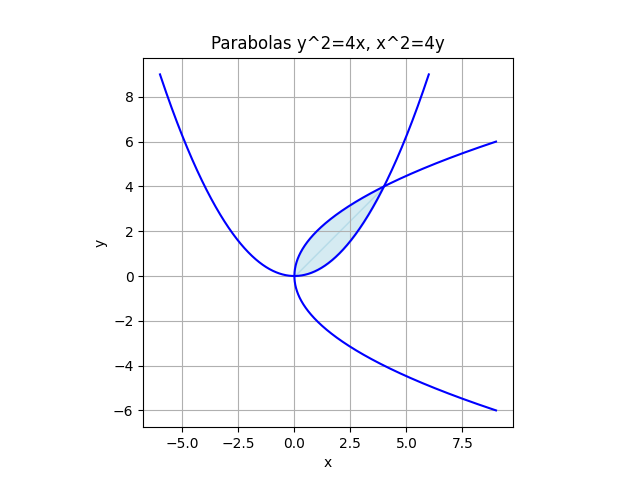
\includegraphics[scale=0.4]{figs/fig.png}
				\label{stemplot}
			\end{figure}
		\end{frame}

		\subsection{Codes}
		\begin{frame}[fragile]
			\frametitle{Codes}
			C Code:
			\begin{lstlisting}[language=C, basicstyle=\scriptsize]
void yparabola_gen(FILE *fptr, double a, double num_points, double **vertex){
	for(int i=num_points; i>=0; i--){
		double t = 3*i/num_points;
		double **output=createMat(2,1);
		output[1][0]=vertex[0][0]+a*t*t;
		output[0][0]=vertex[1][0]+2*a*t;
		fprintf(fptr,"%lf,%lf\n",output[0][0],output[1][0]);
		freeMat(output,2);
	}
	for(int i=0; i<=num_points; i++){
		double t = -3*i/num_points;
		double **output=createMat(2,1);
		output[1][0]=a*t*t;
		output[0][0]=2*a*t;
		fprintf(fptr,"%lf,%lf\n",output[0][0],output[1][0]);
		freeMat(output,2);
	}
}
			\end{lstlisting}
		\end{frame}
		\begin{frame}[fragile]
			\frametitle{Codes}
			\begin{lstlisting}[language=C, basicstyle=\scriptsize]
void xparabola_gen(FILE *fptr, double a, double num_points, double **vertex){
	for(int i=num_points;i>=0;i--){
		double t = 3*i/num_points;
		double **output=createMat(2,1);
		output[0][0]=vertex[0][0]+a*t*t;
		output[1][0]=vertex[1][0]+2*a*t;
		fprintf(fptr,"%lf,%lf\n",output[0][0],output[1][0]);
		freeMat(output,2);
	}
	for(int i=0;i<=num_points;i++){
		double t = -3*i/num_points;
		double **output=createMat(2,1);
		output[0][0]=a*t*t;
		output[1][0]=2*a*t;
		fprintf(fptr,"%lf,%lf\n",output[0][0],output[1][0]);
		freeMat(output,2);
	}
}
			\end{lstlisting}
		\end{frame}
		\begin{frame}[fragile]
			\frametitle{Codes}
			\begin{lstlisting}[language=C, basicstyle=\scriptsize]
int main() {
	double x1, y1;
	x1 = 0; y1 = 0;
	int m = 2, n = 1;
	double **vertex = createMat(m, n);
	vertex[0][0] = x1;
	vertex[1][0] = y1;
	double radius = 4;
	FILE *fptr;
	fptr = fopen("line_points.txt", "w");
	if (fptr == NULL) {
		printf("Error opening file!\n");
		return 1;
	}
	double a = 1;
	yparabola_gen(fptr, a, 1000,vertex);
	xparabola_gen(fptr, a, 1000,vertex);
	fclose(fptr);
	return 0;
	}
			\end{lstlisting}
		\end{frame}
		\begin{frame}[fragile]
			\frametitle{Codes}
			Python Code:
			\begin{lstlisting}[language=Python, basicstyle=\scriptsize]
import numpy as np
import matplotlib.pyplot as plt
points = np.loadtxt("line_points.txt", delimiter=',', max_rows=len(list(open("./line_points.txt"))))
centre=np.array([points[0][0],points[0][1]])
x1 = points[:2002, 0]
y1 = points[:2002, 1]
x2 = points[-2002:,0]
y2 = points[-2002:,1]
plt.figure()
plt.plot(x1, y1, label='y^2=4x', color='blue')
plt.plot(x2, y2, label='x^2=4y', color='blue')
plt.fill_between(x2, y1, y2, where=(y2 >= y1), color='lightblue', alpha=0.5)
plt.fill_between(x1, y1, y2, where=(y2 >= y1), color='lightblue', alpha=0.5)
plt.gca().set_aspect('equal', adjustable='box')
plt.xlabel("x")
plt.ylabel("y")
plt.grid(True)
plt.show()
			\end{lstlisting}
		\end{frame}
	\end{document}

